\section{Robust Testing of Complete Coloring Laws}
\label{sec:robust-laws}
The previous 183 rejections concern a calibrated but potentially insensitive
instrument. We audited all 795 historical results and reproduced all 100
known-star control $p$-values exactly. The original 19,999 permutations give
$p_{\min}=0.00005<0.05/795$; Holm resolution was sufficient. Characteristicness
of the Hamming kernel does not imply useful finite-sample power.

On the 201-vertex star, let leaves be independent uniform binary colors and
let the independent center be uniform on 199 high colors under $P$, versus
a 100-color subset under $Q$. Every vector is a proper local-list coloring.
Writing $a=e^{-1/201}$ and $b=(1+a)/2$ gives
\[
 \operatorname{TV}(P,Q)=99/199,\qquad
 \operatorname{MMD}^2=b^{200}(1-a)(1/100-1/199)
 \simeq1.5021\,10^{-5}.
\]
Under $P=P$, the kernel row mean is constant. If
$\zeta_2=\mathbb E[k^2]-(\mathbb E k)^2$, then the equal-size unbiased
statistic has exact variance
$[4/(m(m-1))+4/m^2]\zeta_2$. At $m=250$, its null standard deviation is
$2.4129\,10^{-4}$: the population signal is only $0.0623$ null standard
deviations. The named event that the center is at most 101 has probability
gap $99/199$ and discards irrelevant leaves.

\paragraph{An honestly selected omnibus.}
We split each independent sample into selection and evaluation halves.
Selection learns local categorical/threshold witnesses, pair and triple
features, structural summaries, a dense marginal score, and empirical
kernel witnesses at $\gamma\in\{.25,1,4,16\}$. An all-pair covariance search
on selection data extends fixed interaction regions. Evaluation uses the
maximum of pooled-standardized mean differences and an always-retained
characteristic full-vector MMD component. Selection never sees evaluation
labels; vertex and color labels are preserved.

\begin{proposition}[Conditional level of the honest maximum]
Under equality of the two output laws, conditioning on selection data and
pooled evaluation observations makes source labels uniformly exchangeable.
Recomputing the entire maximum under fixed-size label permutations, using
inclusive ties and the plus-one rule, yields a superuniform $p$-value.
\end{proposition}
\begin{proof}
The selected functions and pooled scales are fixed under this conditioning.
Uniform allocations therefore give the statistic's conditional null law.
The inclusive upper rank of the observed allocation among uniformly drawn
allocations is superuniform; averaging over the conditioning variables
preserves this inequality. Maximization is included in every allocation,
so it introduces no additional uncorrected search.
\end{proof}
Full finite-space arguments, consistency and computational-futility bounds
are given in the accompanying theory. Our global multiscale max/softmax
benchmarks are explicit adaptations inspired by MMDAgg and MMD-FUSE
\citep{schrab2023mmdagg,biggs2023mmdfuse}; we do not transfer their continuous
Sobolev minimax claims to discrete coloring spaces. Conditional random-rank
calibration follows the finite permutation framework
\citep{hemerik2018exact,phipson2010permutation}.

\paragraph{Independent instrument validation.}
Proper-coloring controls cover localized marginal changes, equal-marginal
dependence, higher-order parity, structural shifts, diffuse bias, rare mass
and huge supports. Null laws include point masses, uniform/discrete laws,
noisy stars, clique symmetry, Luby/Luby and actual checkpoint/self draws.
Each null law has 400 independent trials. Alternative grids use 30 trials
at $m=100,250,500,1000,2000$, counting selection observations in $m$.
The first version missed relocated pairs; a training-only pair search was
then validated with fresh second-round data before neural confirmation.
The final instrument passed its prespecified calibration and power gate.
The known-star alternative was detected in 30/30 independent trials at
both $m=250$ and $500$, even at $0.05/795$ with 19,999 permutations;
the pointwise Wilson lower power bound is $0.886$. Unknown remote triples
and sufficiently rare events remain sensitivity limitations, preserved
in the reported curves. No universal finite-sample power is claimed.

\begin{figure}[ht]
\centering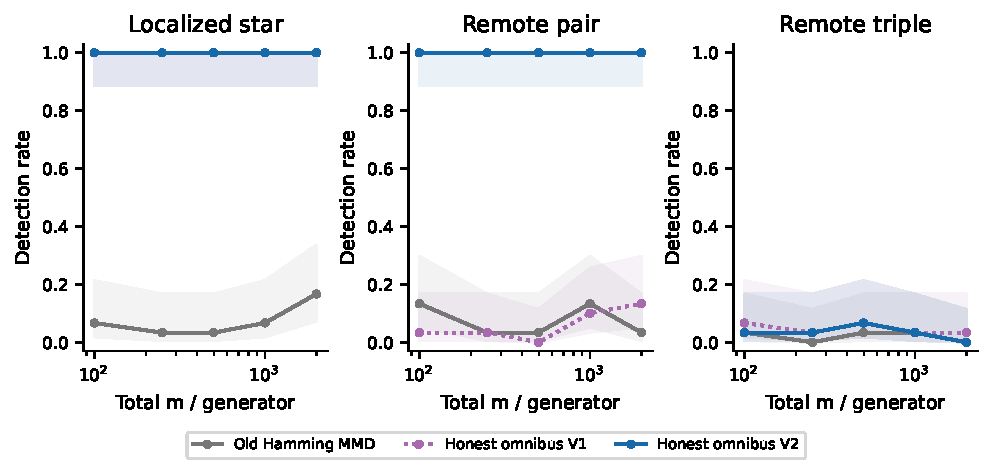
\includegraphics[width=\linewidth]{figures/robust-power.pdf}
\caption{Selected independent second-round controls. Each total sample budget
includes the selection half. Bands are pointwise Wilson 95\% intervals
over thirty independent trials. Remote higher-order alternatives
retain failures; the known TV alone does not determine power.}
\end{figure}

An independently prespecified post-freeze replication investigated the noisy-star null after its original 32/400 rejections. The unchanged omnibus rejected 202/4000 independent null trials (rate 0.0505; pointwise Wilson 95\% interval [0.0441,0.0577]). This diagnostic neither replaced the original gate nor selected a new procedure.

\paragraph{Fresh frozen-policy confirmation.}
The final protocol was committed after instrument validation and before
generating new comparison banks. It retains the same 53 historical graph
entries (51 unique labeled graphs), all fifteen recent epoch-120 policies,
local lists and independent execution streams. Primary tests use 500 runs
per generator: 250 selection and 250 evaluation when all runs complete.
Conditional tests use only proper completions in that fixed prefix and
record their effective selection/evaluation counts if a cutoff occurs.
The old MMD uses all proper completions in the same fresh prefix.
Holm controls each planned 795-test
family at 0.05. The historical 250-run result is preserved separately.

The robust primary family rejected 340/795 hypotheses; the old test on the same fresh 500-run banks rejected 239/795. Of E1's 255 historical nonrejections, 42 reject under the new procedure. Changes from history combine method, sample budget and fresh sampling; matched-budget comparisons and independent controls are needed to assess sensitivity.
The matched primary comparison contains 104 new-only and 3 old-only rejections. The new instrument does not dominate every alternative: in the auxiliary Transformer cohort at total m=2000 it rejected 20/45 cells versus 24/45 for the old MMD. These are nested-sample decisions, not estimates of alternative-specific power.
The full fresh confirmation allocation recorded 2,867,996 valid completions, 0 invalid complete outputs, 4 cutoffs and 0 technical errors. Cutoffs are retained as operational outcomes; they are not replaced by additional draws. Conditional clique symmetry does not imply identical termination probabilities.
\begin{center}
\begin{tabular}{lrrr}\toprule
Architecture & Historical 250 & Old, fresh 500 & New, total 500\\\midrule
NORMALIZED (E1) & 10 & 21 & 52\\
DeepSets & 46 & 71 & 107\\
LocalPaletteTransformer & 127 & 147 & 181\\
\bottomrule\end{tabular}
\end{center}
All counts are rejections among 265 fixed graph--checkpoint cells, not
distributional distances. Complete negative results and checkpoint-specific
effects are archived. Auxiliary sample-size comparisons use a separate
405-hypothesis family on nine prespecified entries. Conditional success
frequencies, all invalid outputs, cutoffs and technical errors remain
separate outcomes.

\paragraph{Independent witnesses and small-space inference.}
After primary selection, the last 250 separately reserved runs per generator
estimate one binary event per cell. Simultaneous Clopper--Pearson intervals
cover all 1,590 event probabilities, and explanatory Fisher tests have their
own Holm family. They identify predictive observables rather than causal
mechanisms. Small graphs additionally use rational teacher laws,
permutation-calibrated categorical likelihood ratios and simultaneous TV
intervals from 20,000 runs per generator, including the teacher
cutoff/eventual-law discrepancy and a conservative float64 rank bound.
The prospective TV tolerance 0.05 was supported in 78/105 small-graph policy cells. This is approximate conditional equivalence at a stated tolerance, not exact equality or a claim for large graphs.
All 35/35 small E1 cells met this criterion (largest simultaneous upper TV bound 0.0437), versus 31/35 for DeepSets and 12/35 for Transformer.
For a contrasting large-graph E1 example, normalized-s41000 on regular-n512-d100 has a selected event that the number of used colors is at most 100. Its independent probabilities are 0.008 under Luby and 1.000 under E1; the simultaneous difference interval is [0.894,1.000]. Hence complete-vector conditional TV is at least 0.894 at the simultaneous coverage level. These selected predictive witnesses are not causal explanations, and no localized E1 witness passed the independent explanatory criterion.
\begin{figure}[ht]
\centering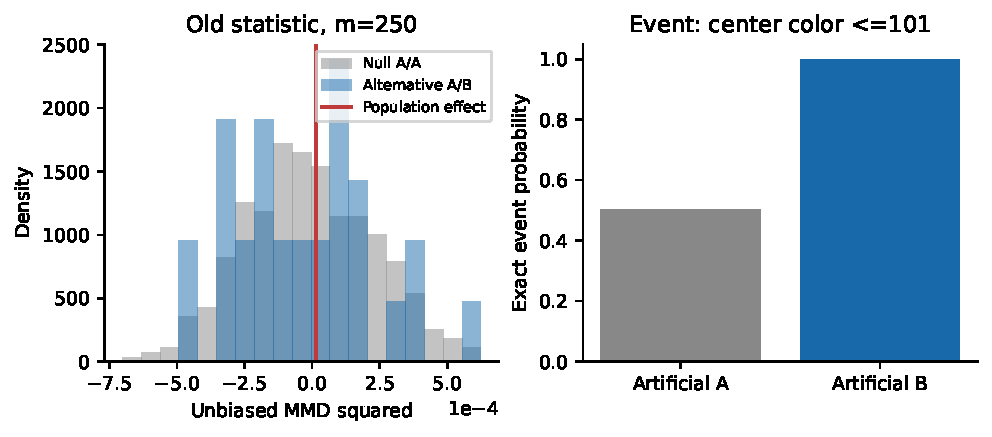
\includegraphics[width=\linewidth]{figures/robust-star.pdf}
\caption{Why large TV can coexist with weak old-MMD power. Left: the old
statistic under independent known-null and known-alternative draws, and its
tiny population effect. Right: the exact localized event probability
gap that an honestly selected witness can preserve.}
\end{figure}

\paragraph{What remains unknown.}
Clique equality follows from ideal vertex symmetry conditional on success;
finite hardware probes do not prove bitwise equivariance. Other neural
laws generally remain algebraically unknown. Nonrejection does not establish
equality, and a small MMD does not imply a useful TV bound without an
appropriate quantitative inequality. Rare-event coupling and large-support
mixtures supply explicit finite-sample lower bounds in the theory document.
The new instrument mitigates verified power failures for named alternatives;
its uncovered interactions are retained as limitations. No universal degree
trend or population statement over graph seeds or training procedures follows.
